\documentclass[border=15pt]{standalone}
\usepackage{amsmath,amssymb,mathtools}
\usepackage{tikz}
\usepackage{pgfplots}
\usepackage{pgf}
\begin{document}
	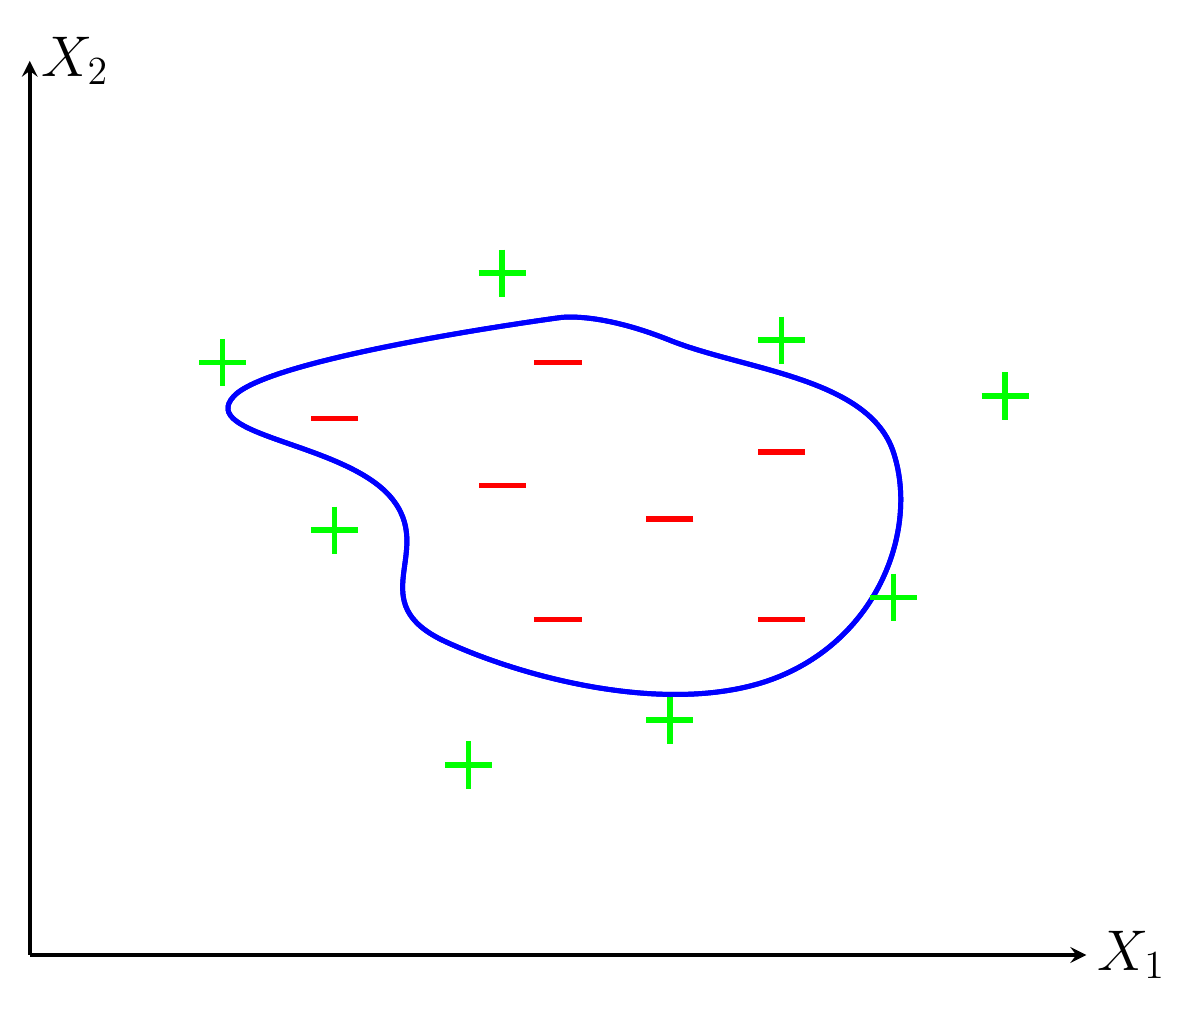
\begin{tikzpicture}
		\begin{axis}[
			xmin=1,
			xmax=9,
			ymin=1,
			ymax=9,
			axis equal,
			width=15cm,
			axis x line=center,
			axis y line=center,
			xmajorticks=false,
			ymajorticks=false,
			ylabel style={right,font=\huge},
			ylabel=$X_2$,
			xlabel style={above,right,font=\huge},
			xlabel=$X_1$,
			line width=1.5pt
			]
			%\addplot[no markers, domain=-1:11]{(5/3)*x};
			
			\addplot[only marks, mark=-,draw=red,mark size=0.3cm,line width=2pt]coordinates {(5,4) (4.5,5.2) (5,6.3) (3,5.8) (7,4) (7,5.5) (6,4.9)};
			\addplot[only marks, mark=+,draw=green,mark size=0.3cm,line width=2pt]coordinates {(8,4.2) (4.5,7.1) (7,6.5) (6,3.1) (4.2,2.7) (3,4.8) (2,6.3) (9,6)};
			\addplot [smooth,tension=0.8,no markers,thick,blue, line width=1.8 pt] coordinates { (5,6.7) (6,6.5) (8,5.5) (7,3.5) (4,3.8)(3.5,5.1) (2.1,6) (5,6.7)};
			\addplot [smooth,tension=0.8,no markers,thick,blue, line width=1.8 pt] coordinates { (5,6.7) (6,6.5) (8,5.5) (7,3.5) (4,3.8)(3.5,5.1) (2.1,6) (5,6.7)};
		\end{axis}
	\end{tikzpicture}
\end{document}